\documentclass[../main.tex]{subfiles}

\begin{document}
	

	\section{SUIT}
	

We contributed to the standardization of software update security mechanism at IETF: the Software Updates for Internet of Things (SUIT) specifications~\cite{ietf2022suit}.
SUIT defines a security architecture, standard metadata and cryptographic schemes able to secure IoT software updates, applicable on microcontroller-based devices.

\subsection{SUIT Workflow}
\label{sec:suit-workflow}

Figure~\ref{fig:suit-workflow}
shows the SUIT workflow.
In the preliminary \emph{Phase~0},
the authorized maintainer %produces and
flashes the IoT device with commissioning material: the bootloader, initial image, and authorized crypto material.
Once the IoT device is commissioned, up and running,
we iterate a cycle of Phases 1-5, whereby the authorized maintainer can
build a new image (\emph{Phase~1}), hash and sign the corresponding
standard metadata (the so-called SUIT manifest, \emph{Phase~2}) and
transfer to the device over the network via a repository (e.g. a CoAP
resource directory). The IoT device fetches the update and
SUIT manifest from the repository (\emph{Phase~3}),
and verifies the signature (\emph{Phase~4}).
Upon successful verification, the new software is installed and booted
(\emph{Phase~5}); otherwise, the update is dropped.


\begin{figure}[t!]
		\centering
%		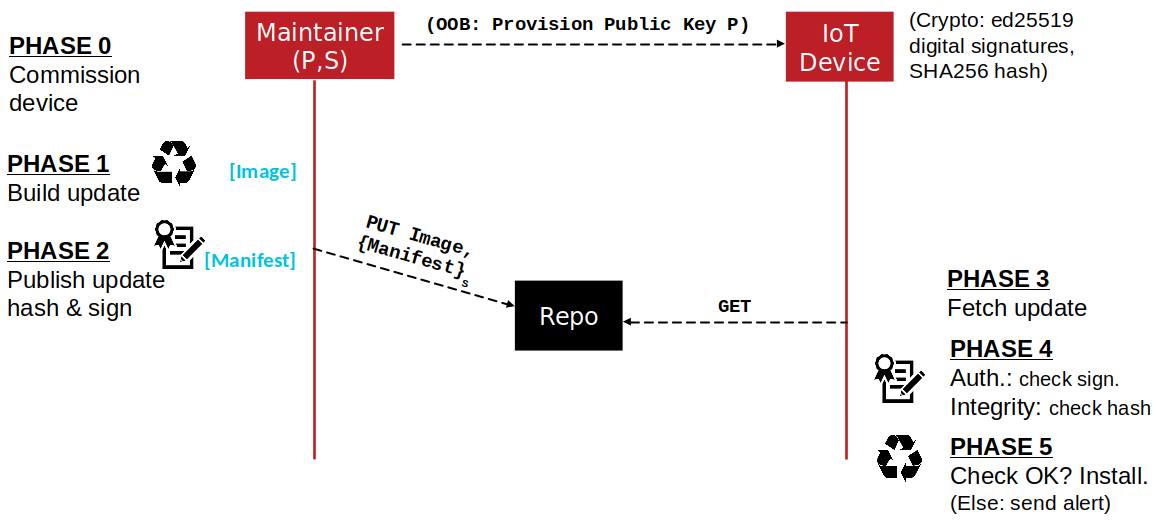
\includegraphics[scale=1]{images/SUIT-workflow.png}
		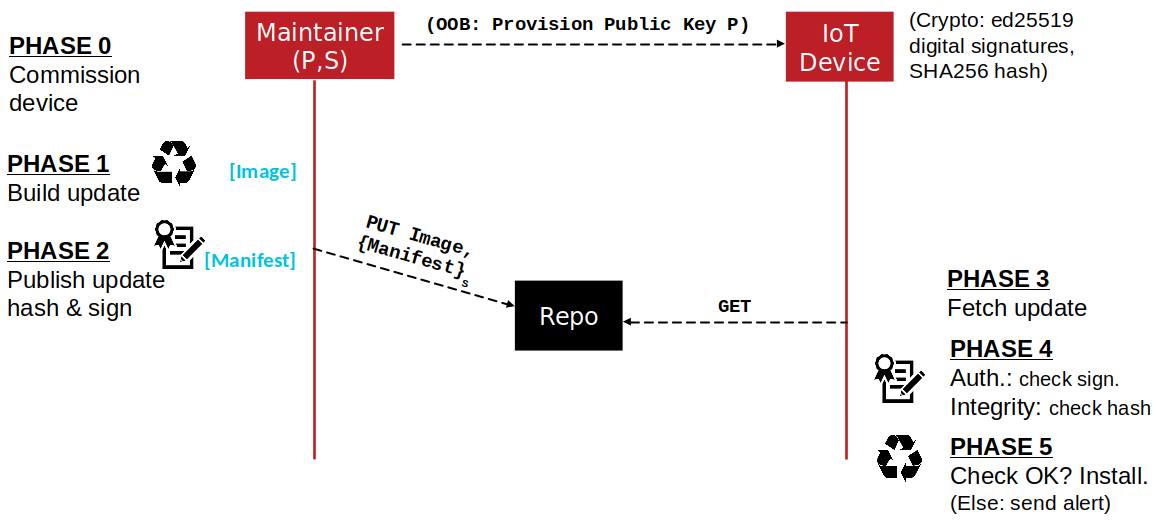
\includegraphics[width=\linewidth]{images/SUIT-workflow.png}
		\caption{SUIT secure software update workflow.}
		\label{fig:suit-workflow}
\end{figure}

%\paragraph{SUIT Cryptographic Tools}
%As depicted in Fig.~\ref{fig:suit-workflow},
The cryptographic tools needed for software updates in general,
and SUIT in particular,
are a digital signature scheme and a hash function.
The digital signature authenticates (a hash of) the software update binary.
To make the signature verification less cumbersome, the signature is not performed on the
software update binary itself, but on a hash of the software update binary.
Thus, this hash function is also a crucial cryptographic primitive in the SUIT workflow.
Fig.~\ref{fig:suit-workflow} depicts this workflow combining SHA-256 hashing and Ed25519 signatures.
Other hash functions, and other signature schemes can be used with SUIT.
For exmaple, in our recent paper~\cite{Banegas2022quantum-suit} we prototyped and comparatively evaluated the use of SHA-3 hashes and quantum-resistant digital signature schemes instead of SHA-256 hashing and Ed25519 signatures (based on pre-quantum elliptic curve cryptography).


\subsection{Security features of SUIT}
The metadata and the cryptographic primitives specified by SUIT can
mitigate attacks exploiting software updates, including:

\begin{itemize}
    \item \emph{Tampered/Unauthorized Software Update Attacks:}
        Adversaries may try to update the IoT device with a modified, intentionally flawed software.
        To counter this threat, SUIT specifies the use of digital signatures
        on a hash of the image binary and the metadata, to ensure the
        integrity of both.
        \item \emph{Unauthorized Software Update Attacks:} An unauthorized party may attempt to update the IoT device with modified software. Using digital signatures and public key cryptography, our prototype based on SUIT ensure that only the authorized maintainer (holding the authorized private key) will be able to update de device.
    \item \emph{Software Update Replay Attacks:}
        Adversaries may replay a valid, but old (known-to-be-flawed) update.
        To mitigate this threat, SUIT metadata includes
        a sequence number that is increased with each new software update.
    \item \emph{Software Update Mismatch Attacks:}
        Adversaries may send an authentic update
        to an incompatible device. To counter this,
        SUIT specifies the inclusion of device-specific
        conditions, to be verified before installing new software.
\end{itemize}
	
	





	
\end{document}